\subsection{Q10.14 data 09202021 10082021 10312021 11092021 grouped by scenario \& group}

\begin{comment}
                        EFPR        EO      EFNR     n    pvalue
(frauth, majority)  0.486111  0.513889  0.500000  36.0  0.993530
(frauth, minority)  0.387500  0.612500  0.425000  40.0  0.095109
(icu, majority)     0.545455  0.454545  0.545455  33.0  0.222079
(icu, minority)     0.403226  0.596774  0.580645  31.0  0.495848
(rent, majority)    0.439024  0.560976  0.378049  41.0  0.457924
(rent, minority)    0.322581  0.677419  0.500000  31.0  0.102470
\end{comment}

\begin{table}[h]
    \centering
    \begin{tabular}{|c|c|c|c|c|c|c|}
        \hline
        scenario & group & EFPR & EO & EFNR & n & p-value\\
        \hline
        frauth & majority & 0.486 & \textbf{0.514} & 0.500 & 36.0 & 0.994\\
		frauth & minority & 0.388 & \textbf{0.613} & 0.425 & 40.0 & 0.095\\
		icu & majority & \textbf{0.545} & 0.455 & \textbf{0.545} & 33.0 & 0.222\\
		icu & minority & 0.403 & \textbf{0.597} & \textbf{0.581} & 31.0 & 0.496\\
		rent & majority & 0.439 & \textbf{0.561} & 0.378 & 41.0 & 0.458\\
		rent & minority & 0.323 & \textbf{0.677} & 0.500 & 31.0 & 0.102\\
		
        \hline
    \end{tabular}
    \caption{Grouped by scenario group}
    \label{tab:my_label}
\end{table}
\begin{figure}[h]
    \centering
    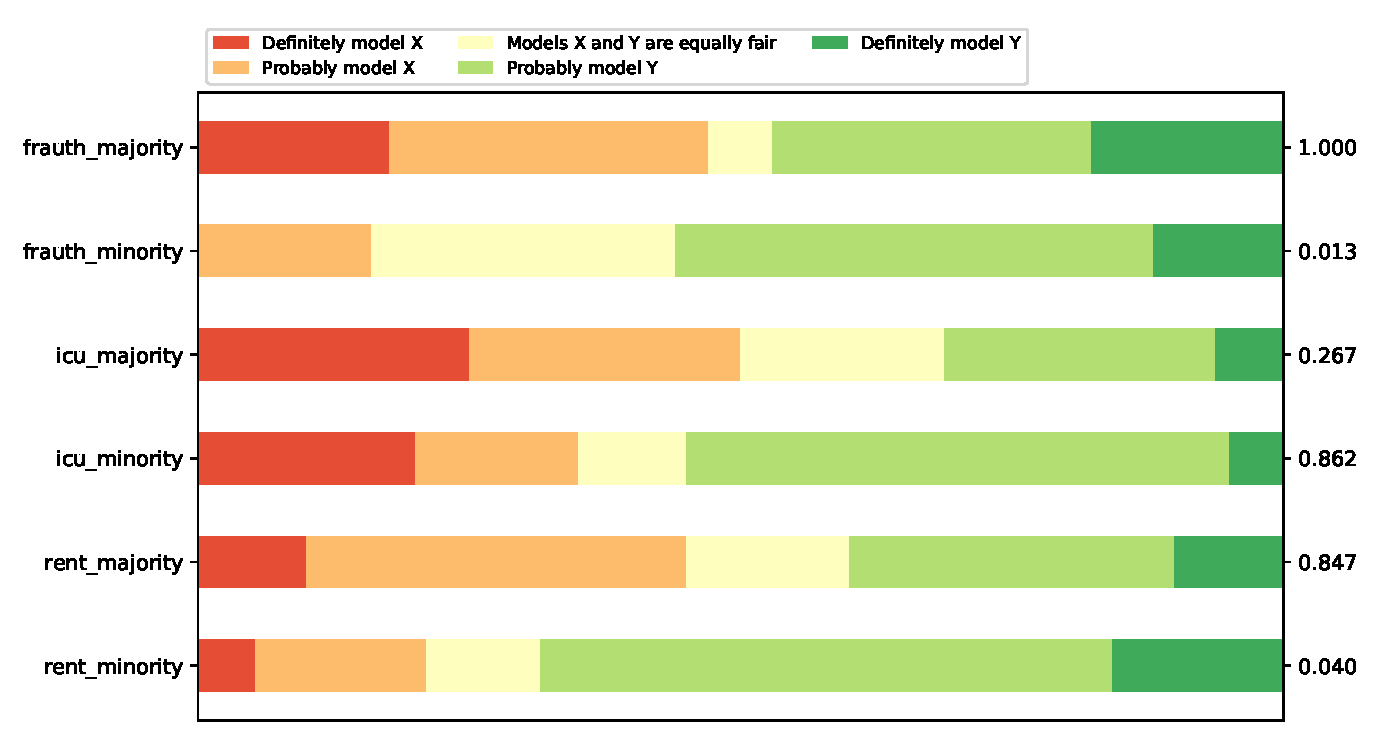
\includegraphics[width=0.8\textwidth]{figures/Q10.14/09202021_10082021_10312021_11092021/Q10.14_scenario_group.pdf}
    \caption{Grouped by scenario \& group}
    \label{fig:my_label}
\end{figure}
